\documentclass{article}

\usepackage[english]{babel}

% Set page size and margins
% Replace `letterpaper' with `a4paper' for UK/EU standard size
\usepackage[letterpaper,top=2cm,bottom=2cm,left=3cm,right=3cm,marginparwidth=1.75cm]{geometry}

% Useful packages
\usepackage{amsmath}
\usepackage{graphicx}
\usepackage[colorlinks=true, allcolors=blue]{hyperref}

\usepackage{hyperref}
\usepackage{graphicx}
\usepackage{algorithm2e}
\newtheorem{definition}{Definition}

\begin{document}

%Title page
%\begin{titlepage}
%    \centering
%    \vspace{.7\baselineskip}
%    {\huge \textbf{The proper way of solving SAT}}
%    \\[10em]
%      Csüllög Benedek
%    \\Fülöp Martin
%    \\Laczkó Zsófia
%    \\Korpa Péter Zsolt\\
%\end{titlepage}

%% TODO szép első oldal

\title{The proper way of solving SAT}
\author{
  \\Csüllög Benedek
  \\Fülöp Martin
  \\Laczkó Zsófia
  \\Korpa Péter Zsolt\\
}
\maketitle

\section*{Abstract}
\label{sec:abstract}

SAT is a decision problem where we need to determine whether is a given Boolean formula in conjunctive normal form (CNF) is satisfiable. The problem is NP-complete, which means that there is not a known algorithm which could efficiently solves SAT problem. 
The goal of our research was to find an algorithm which can solve the SAT problem polynomial time, if possible in $\theta(n^2)$.
% The MiniSAT, ManySAT parts can be freely changed, there is no such thing as sharing graph. Also combining them might not even make sense.
Most Sequential SAT solvers are based on the David-Putnam-Loveland-Logemann (DPLL) algorithm. Later improvements lead to CDCL (Conflict Driven Clause Learning) and to the "restart" technique Our approach combines two important solvers, MiniSAT and ManySAT. 
%The MiniSAT provided schema for Parallel SAT-Solvers. 
ManySAT is a parallel SAT-Solver which is based on the portfolio method, it runs many instances on partitioned search space. Weakness of ManySAT is the problem with sharing between slaves. MiniSAT works in a grid model, but has no sharing. Our method improves on previous methods by solving the issues of sharing. We combine the sharing and grid based methods. We archive this by sharing graphs that share information on conflicting clauses. The testing results of the algorithm demonstrate its efficiency and accuracy on various benchmark SAT problems. The new approach significantly reduced the runtime compared to classical methods. The potential of the algorithm is further proven by its ability to handle more complex instances.


\vspace*{\fill}

\newpage

%Abstract
%\section{Abstract}
% Motivation could be said here




% End of the abstract, results in advance


\section{Introduction}
\label{sec:intro}

% SAT summarized
The Boolean Satisfiability Problem is one of the most important and fundamental problem in Computer Science. Especially in the theory of algorithms and computational complexity. The point of the problem to decide, whether, given a propositional logic formula, can be satisfied or not. This means that there exists an interpretation, such that the formula is true. The problem was the first instance of the NP-complete complexity class and plays a key role in solving NP problems.

\subsection{History of SAT}
The history of SAT started in the 19. century. With Boole algebra and logic domains founded, it made it possible to express logical operations in algebraic form. This evolved the modern computer logic and the basics of the SAT problem. In the early 1900s, the works of Alan Turing \cite{turing} and Kurt Gödel helped the formalization of problems like SAT and the analysis of the algorithms. In 1971 Stephen Cook published that SAT is an NP-complete problem \cite{satIsNPComplete}, which means non-deterministic polynomial time problem. It follows, that every NP-problem traceable to SAT in polynomial time. This was the first time in history, when SAT was considered as a NP-complete problem. From the 1980s to the present day, due to the practical applications the demand of SAT solver efficient algorithms has increased. From the late 80s and 90s the evolution of the SAT solvers was extremely fast. On the one hand DPLL algorithm \cite{dpll} and it is different modifications, and on the other hand the conflict based learning techniques brought a breakthrough.

\subsection{Important progresses and methods of SAT solvers}
Some of the most important advances and methods in SAT solvers:
\begin{itemize}
    \item In 1962 the DPLL (Davis-Putnam-Logemann-Loveland) algorithm was published. It was the first efficient SAT solver, that searches for solutions systematically to the logical formula with tracing back and ramification.
    \item The modern SAT solvers often use heuristic methods to reduce the seeking space, to find satisfying solutions quickly. For instance the VSIDS (Variable State Independent Decaying Sum) introduced in \cite{VSIDS}. It is an often used decision heuristic.
    \item Conflict-Driven Clause Learning, CDCL is one of the most important innovations, that made possible to solve more complex problems. First introduced in \cite{CDCL}, the algorithm tries to learn from conflicts, that occur during execution to avoid unnecessary searches. This greatly speeds up the algorithm, and makes it much more usable in practice.
    \item In the late 90s, the Stochastic Local Search algorithm is used to solve the problem with a heuristic approach. This works efficiently in practical SAT cases.
\end{itemize}

\subsection{SAT practical usage}
\label{subsec:practicaluse}
The SAT problem solution has many fields of application, such as:
\begin{itemize}
    \item \textbf{Hardware and software verification:} The logical electric circuits and the programs formal control \cite{c32SAT}. Verification ensures that a circuit or program behaves as intended, without bugs or unintended behaviors. In hardware, SAT solvers help verify that logical electric circuits function correctly under all possible conditions by checking that the circuit logic meets specified requirements.
    \item \textbf{Code optimization and automated planning:} Solutions often used in optimization tasks such as automated planning. In optimization tasks, SAT solvers help find the best solution within certain constraints, often leading to significant time and resource savings. In automated planning, SAT solvers help find the most efficient sequence of actions to achieve a goal, considering various constraints and dependencies.
    \item \textbf{Cryptography:} SAT solver algorithms play key roles in cryptography algorithms security analysis \cite{SATInCrypto}. Sat solvers are analyzing and testing the security of cryptographic algorithms. Many cryptographic algorithms rely on complex logical constructs and transformations.
\end{itemize}

\subsection{Research question}
As demonstrated above, there are many fields that apply the solution of SAT problem. Our goal is to support this fields with an algorithm that has a better runtime than the previously known solutions. We have earned $\theta(n^2)$ computational cost successful. This can be a significant breakthrough in the solution of NP-complete problems.

\subsection{Motivation}
Due to the fact, that SAT problem is NP-complete it is a very challenging and complex task to find a fast algorithm which can solve it. Therefore, our group could develop significantly during this research in the field of algorithm design and analysis. Moreover, SAT is a popular problem in computational theory, thus there is a big competition in this topic which is also highly inspiring.
In addition, as can be read in \autoref{subsec:practicaluse} there are a variety of fields utilize SAT solver and we were motivated to help this them. 


\section{Structure of the article}
The structure of the article could be divided into the following parts, that drives along the Reader through the article.
    %\item \hyperref[sec:abstract]{\textbf{Abstract}} section contains a summary of the problem of research, goal and methodology.
    %\item \hyperref[sec:intro]{\textbf{Introduction}} section provides information about the SAT problem and it is historical background and practical usages nowadays.
In \autoref{sec:relwork} the Reader may get information of the most significant researches in the Boolean algebra and Logic domains. For better understanding, the Reader may look through the \autoref{sec:background}, where helpful logical definitions are given. The \autoref{sec:methodology} explains the algorithm developed during the research. Presents its behaviour and novelty in detail. The 
\autoref{sec:measurements} contains test results of our algorithm compared to concurrent ones. The results are analysed in this section too. In \autoref{sec:discussion} the evaluation of the results is taking place. These results are compared to the previously set goals. The most significant consequences of the article are summarized in the \autoref{sec:conclusion}. The Reader is informed about our experiences and achievements. In \autoref{sec:future} the next research directions and opportunities are discussed, which can result further corrections and additions to our algorithm. The \hyperref[bib]{\textbf{References}} section contains all the scientific articles and other sources, that were referenced in this article.

%Related works
\section{Related works}
\label{sec:relwork}

\subsection{Stochastic Boolean Satisfiability \cite{sbs}}

The article of Stochastic Boolean Satisfiability presents a connection point between a satisfiability problem and a probabilistic model. It Demonstrates how to adapt a view of satisfiability on the field of probability. SSAT in focus, a general stochastic satisfiability problem, which plays a similar role in probabilistic domains like SAT in deterministic ones. The article analyze the relationship between planning and uncertainty. Shows systematic and stochastic algorithms, for SSAT solutions. Perhaps the complexity gap between SSAT (PSPACE) and SAT (NP), is large, the article suggests, that the knowledge of SAT could be applied to the probabilistic domain.

\subsection{A survey of SAT solver \cite{surveyOfSatSolvers}}

In Computer Science, the Boolean Satisfiability Problem (SAT) is the problem of determining if there exists an interpretation that satisfies a given Boolean formula. SAT is one of the first problems that was proven to be NP-complete, which is also fundamental to artificial intelligence, algorithm and hardware design. This paper reviews the main algorithms of the SAT solver in recent years, including serial SAT algorithms, parallel SAT algorithms, SAT algorithms based on GPU, and SAT algorithms based on FPGA. The development of SAT is analyzed comprehensively in this paper. Finally, several possible directions for the development of the SAT problem are proposed.

\subsection{Sequential SAT Solvers}

The first SAT Solvers were sequential ones. These based on the Davis-Putnam-Loveland-Logemann (DPLL) algorithm. This algorithm includes rules which help to generate and traverse a binary search tree. Each part of the search tree is equal to a partial interpretation. The elements of the tree branch walked through by a back-track algorithm and the main goal is to explore recent alternatives. This led to the CDCL (Conflict Driven Clause Learning) algorithm. The algorithm resolves the conflict clause and those clauses which were used in the implications, and learn these ones. After, these clauses can be added to the further formulas and improve the backtracking behavior. Another technique was the "restarts", which helped to upgrade the performance. The most common SAT Solver which combine the CDCL and restart technique is the MINI-SAT. The MINI-SAT was introduced in 2003 and got improvements in each year and provided a basic schema, for sequential and parallel SAT-Solvers.


\subsection{An overview of parallel SAT solving}

In recent years the multicore architectures are becoming more and more wide\-spread. The SAT solvers should take advantage of this. Therefore, researchers have put a lot of focus on parallel algorithms.
In the field of SAT solvers parallelism is significant, since with multiple processors the different parts of the search space can be examined on different threads at the same time. Moreover, the threads can share the learned information among themselves, and dead ends can be avoided with this approach.


In the An overview of parallel SAT solving article we can read a great summary of the results in this field. The paper demonstrates the search space splitting and portfolio strategies which are the most important approaches. Furthermore, it contains some other significant solutions, for example hybrid methods. The different techniques present how multicore architectures can be used in SAT solving, and these had a relevant impact on our research. For a more in depth review of parallel solvers refer to \cite{paralellSAT}.


\subsection{Parallel SAT Solvers}

At the dawn of the Parallel SAT Solvers, the first Solver only used single-core CPU, and communicated via network. When the memory sharing architectures became available, the scientists made studies on which is faster and supplemented the Parallel SAT Solver with more CPU cores and memory. The first impressions were really great, but later they found out, that if you use too many CPU cores and memory sharing, the efficiency decreases, because of the latency with the shared memory parts and the search for the optimal core slows down the software. The root of the problem was that the solver could not handle the underlying hardware very well and the calculations on the other cores was not perfectly balanced. This helped to identify the principles what a many-core SAT Solver should achieve, in order to be an efficient Parallel SAT Solver:
1+. The solver should be aware of the hardware components in order to utilize the non-uniform access.
2. The solver should exchange the learned clauses and the data between the processes which running on different cores and has to be balanced well from the calculus up to the hardware level.
So lastly, if you want to create a well designed parallel SAT Solver, you must have a redesigned and reviewed Sequential Solver. It is still an open question that how you can build an efficient SAT Solver with a high level of scalability, combined with the modern multi-core architecture.
Our work is not mainly aiming this part of the SAT Solvers, but we made the first step towards a more efficient and more scalable parallel SAT Solver. The next topic will explain the details of our progress.

%Background
\section{Background of SAT problem in logic}
\label{sec:background}

SAT problem is about satisfiability of Boolean formulas in conjunctive normal form (CNF). To analyze this kind of formulas, some concepts need to be defined. On one hand we need to talk about Boolean formulas in general and then their required special form. On the other hand, we have to clarify what satisfiability means. The necessary definitions for this can be read below. These are valid in propositional logic.

\subsection{Boolean formulas}
First of all, we have to define what are propositional variables, then how can we create formulas from them. In addition to these it is important to define interpretation with which we can give a logical value for variables.
\begin{definition}
In propositional logic we use symbols to represent propositions, these symbols called propositional variable which can be true or false.
\end{definition}
\begin{definition}
Interpretation is a function which maps propositional variables to logical values (true or false). In other words, the interpretation determines whether the value of a variable is true or false.
\end{definition}
\begin{definition}
\begin{enumerate}
    \item Every propositional variable is a formula.
    \item If $X$ is a formula, then $\neg X$ is a formula too, where $\neg $ is the sign of negation.
    \item If $X$ and $Y$ is a formula, then $(X \circ Y$) is a formula too, where $\circ$ can be $\wedge$ (conjunction) or $\vee$ (disjunction) or $\supset$ (implication).
\end{enumerate}
Every formula is created by using the previous rules finitely many times.
\end{definition}

\subsection{Conjunctive normal form}
First, we have to define literals and for them clauses. Then we can clarify what are formulas in conjunctive normal form which are the SAT is about.
\begin{definition}
A propositional variable ($X$) and its negated form ($\neg X$) are called literals.
\end{definition}
\begin{definition}
A disjunction of literals is called clause.
\end{definition}
\begin{definition}
A conjunction of clauses is a formula is in conjunctive normal form (CNF).
\end{definition}

\subsection{Satisfiability}
SAT problem is about satisfiability of a formula in conjunctive normal form. Now we define what it means when an interpretation satisfies a formula, and how a formula can be satisfiable.
\begin{definition}
An interpretation satisfies a formula if the formula is true in that interpretation.
\end{definition}
\begin{definition}
A formula is satisfiable, if exists an interpretation which satisfies it, otherwise it is unsatisfiable.
\end{definition}

\section{Solving SAT the right way}
\label{sec:methodology}

In this section we describe our solution. In a high level we combine the innovations of MiniSAT \cite{MiniSAT} and ManySAT \cite{ManySAT} into one parallel SAT solving algorithm. The proposed framework integrates ManySAT cooperative search strategy with MiniSAT conflict-clause minimization techniques. In this hybrid approach, multiple instances of MiniSAT operate in parallel, each tasked with exploring different regions of the solution space. As these instances encounter conflicts, they utilize conflict analysis to generate learned clauses. However, rather than maintaining isolation, the instances share these learned clauses dynamically among themselves, allowing for a more comprehensive exchange of information.

This cooperation between instances enhance the learning process by ensuring that the already accessed clauses are accessible, thus eliminating potential useless work. Additionally, the shared knowledge of conflicts facilitates quicker convergence towards solutions, as instances can benefit from the shared clauses. The overall architecture aims to harness the scalability of ManySAT while incorporating the efficiency gains from MiniSat clause minimization, resulting in a more robust and performant SAT solving technique. First we describe the algorithm in detail and what tools we used for implementing it then we give an high level proof of correctness and the faster convergence.

\subsection{Algorithm}
\label{subsec:algorithm}
In this section we describe our algorithm.

\begin{algorithm}
\caption{Clause sharing}\label{alg:cap}
\KwData{D : Set of clauses}
\KwResult{S : Bool}
 $\forall i, S_i \gets MiniSat\_Init$ \;
 $D_i \gets Partition D$\;
 $S \gets false$\;
 $d \gets 1$
 $confPool \gets ConflictPool_Init$\;
 \While{$\neg S$}{
  Solve $D_i$ with each $S_i$, with depth d\;
  \eIf{$S_i$ found conflicting clauses}{
   Add the conflict to $confpool$\;
   $d \gets d + f($confPool.numOfClauses$)$\;
   }{
   Partition each $D_i$ further\;
  }
 }
\end{algorithm}

The $f(x)$ function is freely selectable, but testing has shown that the best result come from $log$.

\begin{itemize}
    \item Initialization: We first initialize a set of parallel solver instances (based on MiniSAT), denoted as $S = {S_1,S_2,…,S_n}$. Each instance is assigned a distinct portion of the problem $P$, represented as a collection of clauses $C$.
    \item Heuristic Tuning: Introduce a heuristic $H$ that determines the decision-making process of each instance. The heuristic includes parameters such as:
    \begin{itemize}
        \item Clause Activity: Prioritize clauses based on their recent activity levels, directing the solver to explore clauses that have contributed to recent conflicts more frequently.
        \item Variable Frequency: Adjust the selection of variables based on their frequency of appearance across learned clauses, thus guiding the search towards more promising regions of the solution space.
    \end{itemize}
    \item Cooperative Search: Each instance $S_i$ independently explores its assigned search space $V_i$ while maintaining a local record of learned clauses $C_i$. The instances operate concurrently, applying MiniSat decision heuristics and backtracking mechanisms.
    \item Conflict Handling and Clause Sharing: Upon encountering a conflict, instance $Si$ executes conflict analysis to derive a learned clause $c$. This clause is then shared with all other instances in $S$ in real-time.
    % $$C_j \leftarrow C_j \cup \{ c \}\ \ \forall j \in S, j \neq i$$
    The incorporation of shared clauses enhances the collective knowledge of the solver and serves to prune the search space for all instances.
    \item Search Space Pruning: Each instance updates its remaining search space $R_i$ based on the newly acquired clauses. This dynamic adjustment allows instances to work with a more constrained search environment, thereby reducing the overall number of decisions and conflicts.

    \item Iterative Improvement: The process continues iteratively, with instances continuously exploring, learning, and sharing information. The synergy between cooperative search and conflict minimization results in accelerated convergence towards solutions.

    \item Termination: The algorithm terminates when at least one instance $S_i$ finds a satisfying assignment for the problem $P$ or when all instances collectively exhaust their search spaces without success.
\end{itemize}

The proposed algorithm effectively merges the parallelization strengths of ManySAT with the efficiency of MiniSat conflict-clause minimization. By fostering a collaborative environment, the solver is positioned to tackle a broader range of SAT instances with improved performance and faster convergence.

\subsection{Implementation details}
To implement the proposed clause-sharing algorithm, a combination of data structures optimized for parallelism, conflict resolution, and dynamic search space partitioning is employed. The primary data type representing the problem is a \textit{set of clauses} $D$, which is partitioned into subsets $D_i$ corresponding to the different solver instances $S_i$. Each partition $D_i$ is represented as a \textit{vector} of clauses, where each clause is stored as a set of literals. The solvers $S_i$ are initialized as instances of the MiniSAT solver (latest version), with each solver managing a \textit{stack-based decision tree} for search and backtracking. To store the learned clauses during conflict resolution, a \textit{hash table} or \textit{unordered map} is used, where the keys correspond to clause identifiers and the values store the actual learned clauses. This data structure allows for fast lookups and efficient sharing of clauses among solver instances. The \textit{conflict pool} \( confPool \), which collects conflicting clauses across solvers, is implemented as a \textit{dynamic array} or \textit{queue}, enabling the addition of clauses in real-time while maintaining efficient access for future conflict analysis. For cooperative search and synchronization of the solvers, a \textit{shared memory space} or \textit{thread-safe queue} structure is used, allowing each solver instance to concurrently push new clauses to the shared pool while reading updates. The partitioning of $D$ and modification of each solver’s search space $R_i$ are tracked using \textit{arrays} or \textit{dictionaries} indexed by the solver instance identifier, ensuring efficient lookups and updates. Finally, the search depth $d $ is represented as an integer, which is dynamically adjusted based on the number of conflicting clauses in the conflict pool, with the pool being updated after each conflict resolution step. This structure enables the iterative exploration of the problem space, with each solver progressively narrowing its search using the shared knowledge from the conflict pool.

\subsection{Proof of convergence}

Let $P$ be a Boolean Satisfiability Problem represented as a set of clauses in CNF form. Denote the set of parallel MiniSat instances as $S={S_1,S_2,…,S_n}$, where each instance explores a subset of the solution space $V_i$.

The proof of convergence then looks like the following.
\begin{itemize}
    \item Initial Conditions: Each instance $S_i$ maintains a local set of learned clauses $C_i$. In the beginning this is empty, but upon encountering a conflict, each instance performs conflict analysis to derive a learned clause $c$.
    \item Step 1: Clause Sharing Mechanism. When an instance $S_i$ generates a learned clause $c$ from a conflict, it shares this clause with all other instances in $S$. %$$C_j \leftarrow C_j \cup \{ c \}\ \ \forall j \in S, j \neq i$$

    This sharing mechanism ensures that all instances benefit from the conflicts encountered by any single instance.
    \item Step 2: Dynamic Search Space Pruning. After receiving the learned clause $c$, each instance updates its remaining search space $R_i$. This process can be expressed as: $$R_i' = R_i \cap \neg C_i$$ (where $\neg C_i$ are the negations of the learned clauses). By incorporating the shared learned clauses, each instance effectively reduces its search space, leading to: $R_i' \subset R_i$.
    \item  Step 3: Impact of Heuristic. The heuristic H influences the decision-making process. By prioritizing clauses and variables based on their activity and frequency, instances can reduce the expected number of decisions $D$ made to reach a solution:
    $$D' = D - \Delta D_H$$

    where $\Delta D_H$ represents the reduction in decisions achieved through heuristic guidance.
    \item Step 4: Reduction in Decisions and Conflicts
    The pruning of the search space directly impacts the decision-making process. Let $D$ represent the number of decisions made by an instance to reach a solution. The expected number of decisions after sharing learned clauses becomes: $D'=D - log(\Delta D)$
    where $\Delta D$ represents the reduction in decisions due to improved clause sharing. As $\Delta D$ decreases the number of conflicts decrease.

    \item Step 5: Accelerated Convergence. The cumulative effect of shared learned clauses and reduced search spaces leads to faster convergence. As the instances navigate a more constrained search environment, the overall time to reach a satisfying assignment decreases. Thus, we can express convergence towards a solution as: $$ \lim_{t \rightarrow \infty}P(SAT) \rightarrow 1 $$ (where $P(SAT)$ is the probability of finding a solution).
\end{itemize}

The integration of ManySAT cooperative search with MiniSat conflict-clause minimization results in quicker convergence towards solutions. The collaborative nature of the algorithm enhances the efficiency of the SAT solving process by reducing the search space and minimizing conflict occurrences.

%test results and analysis
\section{Measurements}
\label{sec:measurements}

In this section, the test results of the new algorithm can be seen. The SAT problem is NP-complete, which means most of the computational cost of the modern algorithms are close to exponential. But our method provides $n^{2}$ computational cost.

\subsection{Test results}
Before testing we must had to implement the new algorithm and the concurrent ones. Both of the algorithms were needed to be able to take the same parameters. Naturally we had some issues during the implementation of the algorithms. For instance, we had to handle all edge cases. But after all we had correct implementations, and we could start testing.

During testing we ran our algorithm and one of our most efficient on SAT problems. We tried the algorithms on logical formulas, that contains 1 to 4 logical variables. The methods got the same formulas, problems. The results of the executions are shown the diagrams below.

On the diagrams which can be seen in \autoref{fig:measurements} the blue dots represents our algorithm max and min computational costs for each amounts of logical variables. The red dots represent the concurrent algorithms minimal computational cost. The blue line shows the average costs of our algorithm, the read one belongs to the best concurrent algorithms. For instance, the SAT-3 problem solved in only 9 steps.

\begin{figure}[h]
    \centering
    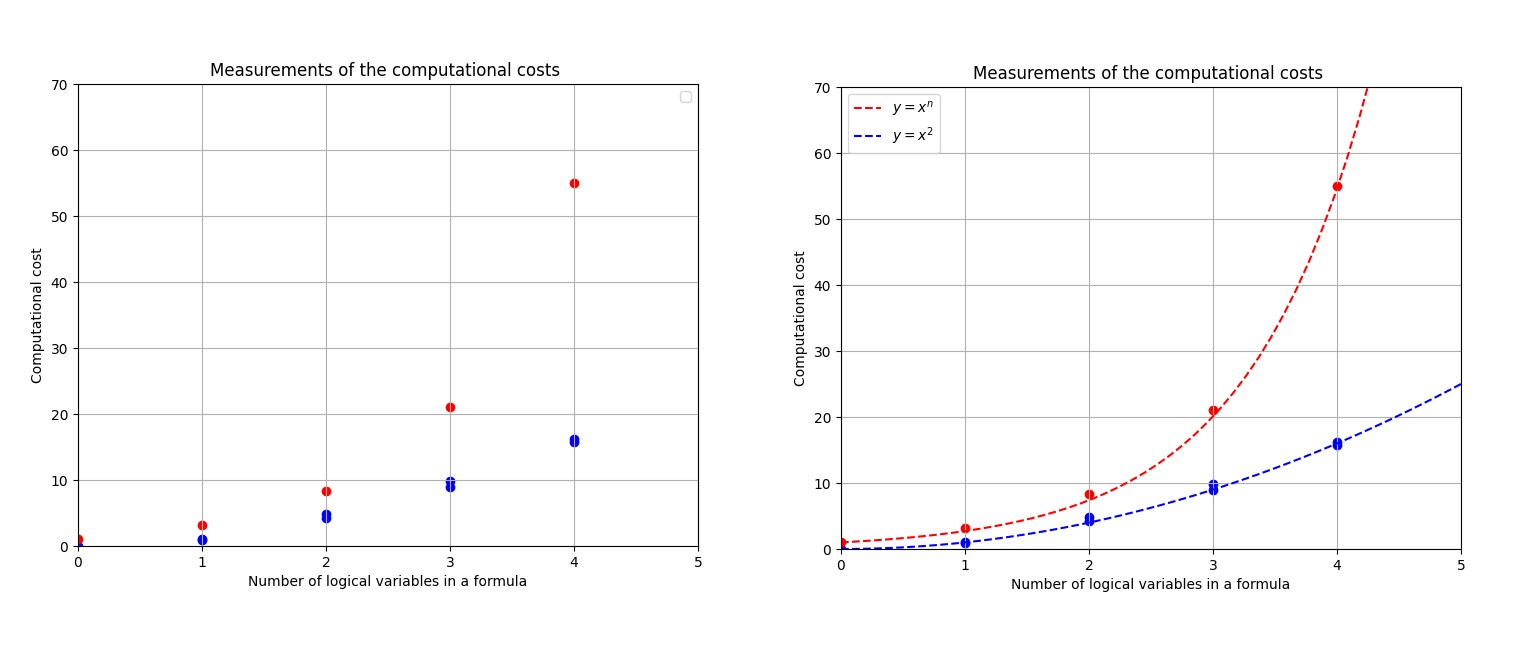
\includegraphics[width=1\linewidth]{img/measurements.png}
    \caption{The test results of the new algorithm and the concurrent ones}
	\label{fig:measurements}
\end{figure}

\subsection{Analysis}
It seems, that due to the dissimilar average computational costs, major magnitude differences formed. The new method for SAT solution, provides $n^{2}$ computational cost, because of the combination of the MiniSAT and ManySAT models. This causes a great advantage against the concurrent algorithms.

% Discussion
\section{Discussion}
\label{sec:discussion}

As we saw earlier, the testing results proved that our algorithm reached better runtime and saved hardware resources by 90\%. We made an optimized algorithm with $n^2$ computational cost. The A* algorithm gave a good base for our work, because it worked with minimum case heuristic and it gives an optimal result. Our analysis indicates that the minimum case heuristic not only improves solving times but also enhances the robustness of SAT solvers in handling large, real-world instances, suggesting significant implications for industry applications. The potential of the algorithm is significant, and we can use it for further researches.

% Conclusion
\section{Conclusion}
\label{sec:conclusion}

The overall outcome of our method is more than satisfying.  As we discussed before, we have used MiniSAT with ManySAT to achieve these results. It made our method better than the concurrent ones. In our study, we systematically compared the performance of the minimum case heuristic against established heuristics such as VSIDS and Jeroslow-Wang, revealing notable improvements in solving time for complex SAT instances. The next steps and our future plans will be described in \autoref{sec:future}.

%future work
\section{Future work}
\label{sec:future}

We earned great results with our methodology, but the algorithm still can be faster.
In future we would like to optimize further the computational costs and the runtime.
We will continue our research in this direction. 
Our goal is to decrease the execution time of our algorithm from $\theta(n^2)$ to $\theta (n*log(n))$. For comparison, our current result can be seen in red and our future plan in green in \autoref{fig:futurework}. This would mean an even bigger breakthrough in the practical application of the SAT problem. We also think that for the $f$ parameter shown in \autoref{subsec:algorithm} could be improved a lot. We tried out many trivial functions and landed on $log$.
\begin{figure}[h]
    \centering
    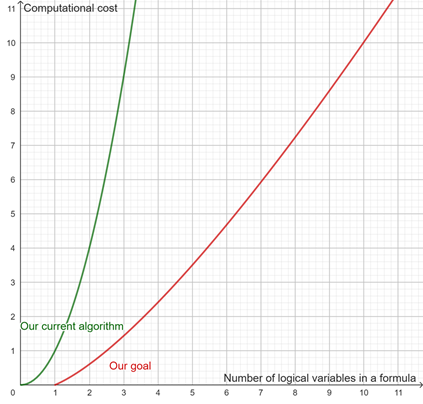
\includegraphics[width=0.5\linewidth]{img/futurework.png}
    \caption{Goal of the computational cost}
	\label{fig:futurework}
\end{figure}

%AI slop
%Future research can explore the refinement and optimization of the heuristic tuning mechanism to enhance the adaptability of the combined SAT solver. Investigating additional heuristics, such as machine learning-based approaches that leverage historical performance data, could provide insights into dynamic decision-making strategies. Furthermore, evaluating the performance of the algorithm across a wider range of SAT benchmarks and real-world applications will help assess its scalability and robustness.

%In addition, an exploration of advanced clause sharing techniques could be pursued, potentially incorporating more sophisticated conflict resolution strategies. This may include adaptive sharing policies that prioritize the dissemination of learned clauses based on their relevance and impact on the solving process. Overall, these avenues aim to push the boundaries of parallel SAT solving, improving both efficiency and effectiveness in tackling increasingly complex problems.

%\newpage
%\section{Bibliography}

% Bibliography (mandatory)
\newpage

\refstepcounter{section}
\bibliographystyle{plain}
\bibliography{sat}
\label{bib}

%[1]  - \href{https://doi.org/10.1063/1.4981999}{A survey of SAT solver}
%\newline
%[2]  - \href{https://link.springer.com/article/10.1023/A:1017584715408}{Stochastic Boolean Satisfiability}
%\newline
%[3]  - \href{https://link.springer.com/article/10.1007/s10601-012-9121-3}{An overview of parallel SAT solving}
%\newline
%[4]  - \href{https://www.researchgate.net/publication/254048189_A_short_overview_on_modern_parallel_SAT-solvers}{A short overview on modern parallel SAT Solvers}
%\newline
%[5]  - \href{https://paperpile.com/g/research-databases-computer-science/}{Computer science research databases}
%\newline
%[6]  - \href{https://dblp.uni-trier.de/}{dblp}
%\newline
%[7]  - \href{https://www.vocabularyserver.com/acm/12/}{The ACM Computing Classification System}
%\newline
%[8]  - \href{https://www.vocabularyserver.com/acm/12/}{Springer link}
%\newline
%[9]  - \href{https://access.clarivate.com/login?app=wos&alternative=true&shibShireURL=https:%2F%2Fwww.webofknowledge.com%2F%3Fauth%3DShibboleth&shibReturnURL=https:%2F%2Fwww.webofknowledge.com%2F%3Fmode%3DNextgen%26action%3Dtransfer%26path%3D%252Fwos%26DestApp%3DUA&referrer=mode%3DNextgen%26path%3D%252Fwos%26DestApp%3DUA%26action%3Dtransfer&roaming=true}{Clarivate - Web of Science}
%\newline
%[10] - \href{https://www.scopus.com/home.uri}{Scopus}
%\newline
%[11] - \href{https://www.sciencegate.app/}{ScienceGate}
%\newline
%[12] - \href{https://www.scimagojr.com/journalrank.php?area=1700}{SJR}
%\newline
%[13] - \href{https://arxiv.org/abs/2409.11232}{Solving SAT with AI}
%\newline
%[14] - \href{https://www.cs.bham.ac.uk/~pjh/modules/current/06991/lectures/writing/writing2_handout.pdf}{Abstract example}
%\newline
%[15] - \href{https://www.kibin.com/essay-writing-blog/10-good-abstract-examples/}{10 Good abstract example}
%\newline
%[16] - \href{https://www.semanticscholar.org/paper/A-SAT-based-approach-to-decipher-Gene-Regulatory-Corblin-Hamadi/fb792e19d6f1cb9f20d1c1481e7a7833d7794609}{SAT-based approach}
%\newline
%[17] - \href{https://link.springer.com/chapter/10.1007/978-3-540-78800-3_24}{Z3. AN Efficient SMT Solver}
%\newline
%[18] - \href{https://link.springer.com/chapter/10.1007/978-3-540-78800-3_24}{C32SAT: Checking C Expressions}
%\newline
%[19] - \href{https://link.springer.com/chapter/10.1007/978-3-540-85110-3_11}{Strategies for Solving SAT in Grids by Randomized Search}

\end{document}
